\chapter{Validaci�n y an�lisis de resultados}\index{Validaci�n}

\section{Modelo Estructural}\index{Modelado!Modelo Estructural}

El dise�o se hizo con la ayuda de algunas referencias, como una tesis de la Universidad Libre de Berl�n en Alemania, en donde se reporta un proyecto muy parecido al presentado en esta tesis, otras referencias son kits de robots que se venden comercialmente y que presentan algunas de las  caracter�sticas que se plantean en el proyecto.\\

La elecci�n en cuanto al material fue el aluminio, ya que presenta caracter�sticas que  benefician la etapa de construcci�n, por ejemplo: es maleable, f�cil de maquinar, ya sea en un maquinado con arranque de viruta o sin arranque de viruta; su densidad es baja, lo que resulta en un peso bajo, es f�cil de conseguir y relativamente barato.\\


 textte xtetextetetxtetset texttextet extetetxtetset
texttex te textetetxtetset texttextet extet texttextet extetetxtet setet xtetset textte
xtetextetetxtetset texttextet extetetxtetset texttex te textetetxtetset texttextet extet texttextet
extetetxtet setet xtetset




 textte xtetextetetxtetset texttextet extetetxtetset
texttex te textetetxtetset texttextet extet texttextet extetetxtet setet xtetset textte
xtetextetetxtetset texttextet extetetxtetset texttex te textetetxtetset texttextet extet texttextet
extetetxtet setet xtetset


\section{Modelado Matem�tico }\index{Modelado!Modelado Matem�tico}
En el modelo matem�tico se encuentran incluidos todos los factores que intervienen en el comportamiento del robot y dependiendo del tipo de modelado, se puede obtener una simulaci�n del comportamiento real del robot.\\

La cinem�tica estudia el movimiento de alg�n sistema sin tomar en cuenta las fuerzas externas que producen este movimiento o que pudieran afectarlo. En el caso del estudio cinem�tico del robot, se describe su movimiento de manera anal�tica mediante una funci�n que relaciona la posici�n y orientaci�n del punto final del robot con los valores de cada una de las articulaciones del robot. Existen dos tipos de estudios cinem�ticos: Cinem�tica Directa y Cinem�tica Inversa.\\

El problema cinem�tico directo se refiere a expresar la posici�n y orientaci�n del punto final del robot a partir de los valores conocidos de las articulaciones.\\

El problema cinem�tico inverso consiste en conocer los valores que se le deben asignar a cada una de las articulaciones para llegar a la posici�n y orientaci�n deseada.\\

La cinem�tica del robot se representa con la llamada Matriz de Transformaci�n Homog�nea. Esta matriz representa la posici�n y la orientaci�n relativa entre dos eslabones seguidos o unidos. Para trabajar con esta matriz es necesario establecer un sistema de coordenadas. Una herramienta muy utilizada para la descripci�n cinem�tica de robots es el algoritmo de Denavit-Hartenberg (D-H). Con la utilizaci�n de esta herramienta se modela cinem�ticamente el robot. El robot tiene un total de 10 grados de libertad divididos en 5 para cada pierna, sin embargo, las piernas son iguales f�sicamente y su movimiento es similar, as� que en realidad s�lo es necesario modelar una pierna de 5 grados de libertad. \\

Los par�metros a utilizar en el algortimo de D-H se muestran a continuaci�n.\\

\newpage

\begin{figure}[h]
	\centering
		\fbox{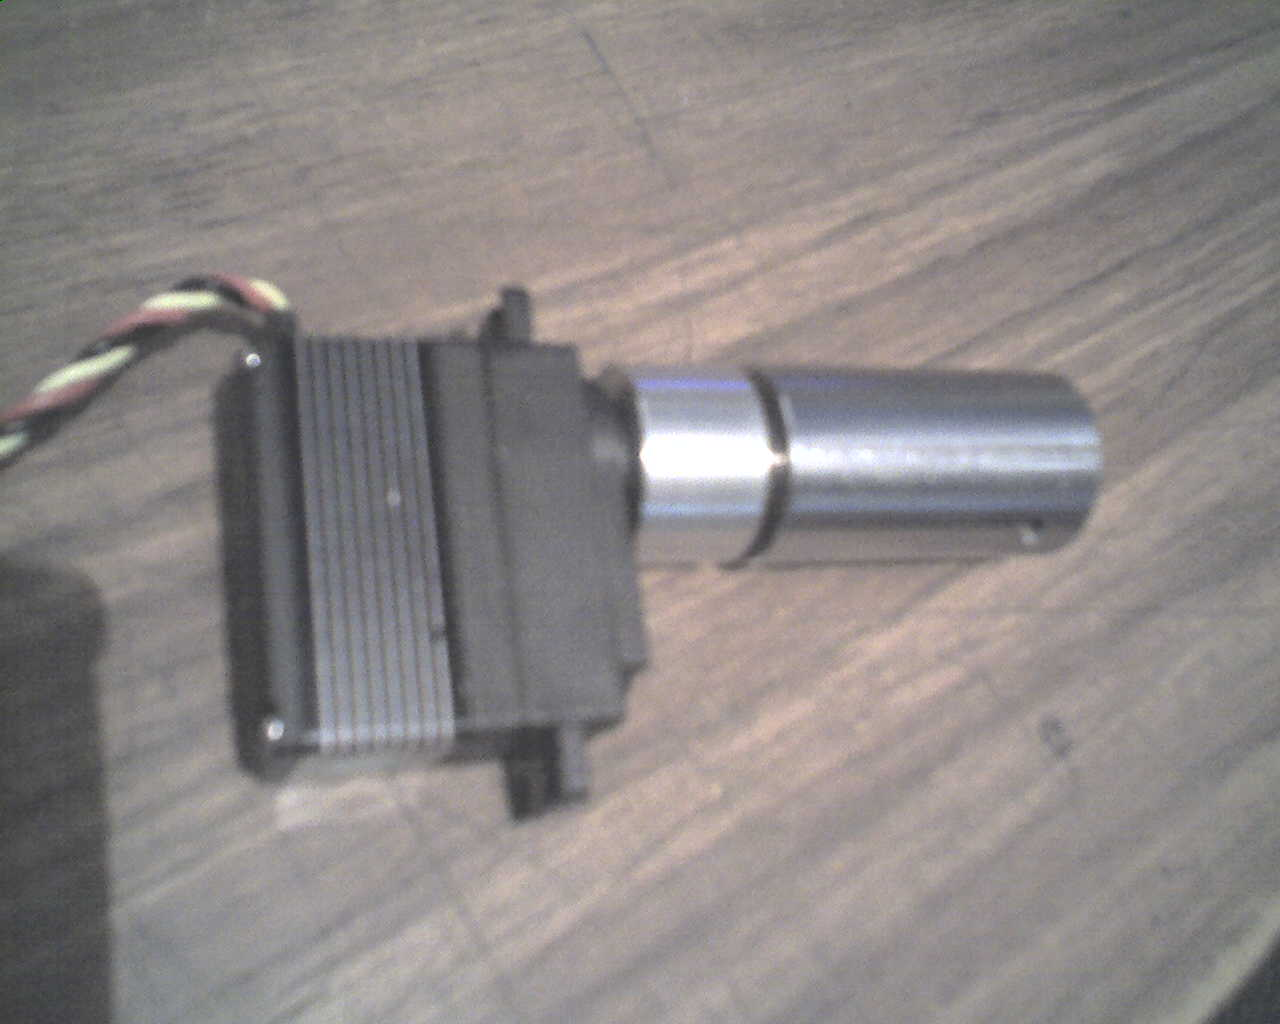
\includegraphics[scale=0.25]{figs/img106.jpg}}
		\caption{Ejes coordenados.}
	\label{fig:DH}
\end{figure}

\begin{table}[h]
	\centering
		\begin{tabular}{|c|c|c|c|c|}
		\hline
			$Eslabon_{i}$	&	$a_{i}$	&	$d_{i}$	&	$\alpha_{i}$ & $\theta_{i}$	\\
			\hline
			0	&	0	&	0	&	0	&	0	\\
			\hline
			1&a1&0&90&q1\\
			\hline
			2&a2&0&0&q2\\
			\hline
			3&a2&0&0&q3\\
			\hline
			4&a1&0&90&q4\\
			\hline
			5&0&0&0&q5\\
			\hline
		\end{tabular}
	\caption{Par�metros de D-H.}
	\label{tab:DH}
\end{table}

Las matrices de transformaci�n Homog�neas obtenidas para cada uno de los eslabones son:\\

\begin{center}

$T_0^1 $= 	\begin{math}
				\left[
				\begin{array}{cccc}
			   	cos(q_1)&               0&         sin(q_1)& 62.82cos(q_1)\\
         sin(q_1)&               0&         cos(q_1)& 62.82sin(q_1)\\
               0&               1&               0&            0 \\
               0&               0&               0&            1

				\end{array}
				\right]
				\end{math}\\
				
\vspace{1cm}

$T_1^2 $= 	\begin{math}
				\left[
				\begin{array}{cccc}
			   	cos(q_2)&	  		 -sin(q_2)&								0&			68.29cos(q_2)\\
          sin(q_2)&          cos(q_2)&                0& 		 68.29sin(q_2)\\
                0&                0&                1&                0\\
                0&                0&                0&                1
				\end{array}
				\right]
				\end{math}\\

\vspace{1cm}				

$T_2^3 $= 	\begin{math}
				\left[
				\begin{array}{cccc}
			   	cos(q_3)&	  		 -sin(q_3)&								0&			68.29cos(q_3)\\
          sin(q_3)&          cos(q_3)&                0& 		 68.29sin(q_3)\\
                0&                0&                1&                0\\
                0&                0&                0&                1

				\end{array}
				\right]
				\end{math}\\
				
\vspace{1cm}				

$T_3^4 $= 	\begin{math}
				\left[
				\begin{array}{cccc}
			   	cos(q_4)&               0&         sin(q_4)& 62.82cos(q_4)\\
         sin(q_4)&               0&         cos(q_4)& 62.82sin(q_4)\\
               0&               1&               0&            0 \\
               0&               0&               0&            1

				\end{array}
				\right]
				\end{math}\\			

\vspace{1cm}

$T_4^5 $= 	\begin{math}
				\left[
				\begin{array}{cccc}
			   	cos(q_5)&	  		 -sin(q_5)&								0&			0)\\
          sin(q_5)&          cos(q_5)&                0& 		 0\\
                0&                0&                1&      0\\
                0&                0&                0&      1

				\end{array}
				\right]
				\end{math}\\
				
				\newpage
				
			
			
{\footnotesize
\begin{center}
				$T_0^5 $= 	
	\begin{math}
\left[
		\begin{array}{ccc}
		\left(\begin{array}{c}
		 cos(q_1)cos(q_5)cos(q_2+q_3+q_4)\\
			   +sin(q_1)sin(q_5)
			   \end{array}\right)&\left(\begin{array}{c}
			   -cos(q_1)sin(q_5)cos(q_2+q_3+q_4)\\
			   +sin(q_1)cos(q_5)
			   \end{array}\right)&cos(q_1)sin(q_2+q_3+q_4\\
			   && \\
\left(\begin{array}{c}
sin(q_1)cos(q_5)cos(q_2+q_3+q_4)\\
-sin(q_1)sin(q_5) \end{array}\right)&\left(\begin{array}{c}
-sin(q_1)sin(q_5)cos(q_2+q_3+q_4)\\
-cos(q_1)cos(q_5)\end{array}\right)&-sin(q_1)sin(q_2+q_3+q_4)\\
   && \\
cos(q_5)sin(q_2+q_3+q_4)&-sin(q_5)sin(q_2+q_3+q_4)&-cos(q_2+q_3+q_4)\\
 & & \\
0&0&0
		\end{array}
				\right]
				\end{math}\\
\end{center}
}
\end{center}

Con este modelo matem�tico es posible generar trayectorias y as� analizar la etapa de caminado. Tambi�n es posible realizar un control de movimiento, sin embargo, este control no ofrecer� la mejor soluci�n, ya que al resolver el problema cinem�tico, no se est�n considerando algunos factores que podr�an afectar al modelo, es por eso que se decide realizar tambi�n un modelado din�mico del sistema.


chos de los sistemas de control que requieren la atenci�n de los
ingenieros son grandes, complejos e involucran muchas variables.
Estos factores est\'an relacionados entre s\'i en modelos
matem\'aticos complicados; las respuestas cuantitativas a estos
problemas se obtienen de soluciones n\'umericas de las ecuaciones
del modelo.

Adem�s de este enfoque para el an\'alisis, es necesario realizar
una investigaci\'on cualitativa simplificada que proporcione
respuestas simples del tipo "si o no'' y que sirvan como una
gu\'ia tanto en el an\'alisis como en el dise\~no.

Las preguntas que se realizan un ingeniero al dise\~nar un sistema
son del tipo: ?`Flotar\'a en barco o se hundir\'a? ?`Se
mantendr\'a en orbita el sat\'elite? ?`? ?`?� ?`
\section{Conceptos b\'asicos}

\section{Criterios de estabilidad}

\subsection{M\'etodo directo de Routh -- Hurwitz}
\subsubsection{M\'etodo de Mikhailov}
\subsubsection{M\'etodo de Hurwitz}
\subsubsection{M\'etodo de Routh}

\subsection{M\'etodo del Lugar de las Ra\'ices}

\subsection{Criterio de Bode}

\subsection{Criterio de Nyquist}
M\'{E}TODO DE NYQUIST PARA EL AN\'{A}LISIS DE ESTABILIDAD DE
SISTEMAS LINEALES

\bigskip

\begin{itemize}
\item  Sistema en lazo cerrado


%\begin{equation*}
%\includegraphics{lc.bmp}
%\end{equation*}

\item  Funci\'{o}n de Tranferencia del sistema en lazo cerrado
\begin{equation*}
\frac{Y(S)}{R(s)}=\frac{G(s)}{1+G(s)H(s)}
\end{equation*}

\item  El sistema en lazo cerrado es estable si todos los polos de la funci\'{o}n de transferencia de lazo cerrado est\'{a}n en el semiplano
izquierdo del plano complejo, es decir,

\begin{quote}
\text{\textit{que ningun polo de lazo cerrado est\'{e} en el}} \\
\text{\textit{semiplano derecho del plano complejo}}
\end{quote}

\newpage

\item  La funci\'{o}n de tranferencia de lazo abierto es $G(s)H(s),$
\end{itemize}

\begin{equation*}
G(s)H(s)=\frac{Z(s)}{P(s)},\qquad Z(s),\text{ }P(s)\text{
}polinomios
\end{equation*}
\quad\ \quad\ *$\quad G(s)H(s)$ es estrictamente propia, o sea, grado de $%
Z(s)<$grado $P(s)$, ello implica
\begin{equation*}
\lim_{\left| s\right| \rightarrow \infty }G(s)H(s)=0
\end{equation*}

\begin{equation*}
1+G(s)H(s)=1+\frac{Z(s)}{P(s)}=\frac{P(s)+Z(s)}{P(s)}
\end{equation*}


\begin{equation*}
\frac{Y(S)}{R(s)}=\frac{G(s)}{1+G(s)H(s)}=\frac{P(s)G(s)}{P(s)+Z(s)}
\end{equation*}

CONCLUSI\'{O}N 1. \ \ Polos de $G(s)H(s)=$ Polos de $1+G(s)H(s)$

CONCLUSI\'{O}N 2. \ Polos de lazo cerado = ceros $1+G(s)H(s)$

\begin{itemize}
\item  CONCLUSI\'{O}N 3. \ De conclusi\'{o}n 2\newline \index{Estabilidad}
``EL sistema es \emph{estable} $\ $\ si \emph{todos los ceros} \ de $%
1+G(s)H(s)$ est\'{a}n en el \emph{semiplano izquierdo} del plano
complejo o \textit{si ninguno de los ceros de }$1+G(s)H(s)$\textit{\
est\'{a} en el semiplano derecho}''\newpage

\item  $1+G(s)H(s)$ como cociente de polinomios
\begin{equation*}
1+G(s)H(s)=k\frac{\left( s+z_{1}\right) \left( s+z_{2}\right) \cdots }{%
\left( s+p_{1}\right) \left( s+p_{2}\right) \left( s+p_{3}\right) \cdots },%
\text{ }k>0
\end{equation*}
\end{itemize}

\^{O}j\^{O} Recordatorio:

$-z_{1,\text{ }}-z_{2,\text{ }}\cdots $, son los polos de lazo
cerrdo,

$-p_{1,\text{ }}-p_{2,\text{ }}\cdots $, son los polos de lazo
abierto, G(s)H(s).


